\hypertarget{1D__path__integral_8cpp}{}\section{1\+D\+\_\+path\+\_\+integral.cpp File Reference}
\label{1D__path__integral_8cpp}\index{1\+D\+\_\+path\+\_\+integral.\+cpp@{1\+D\+\_\+path\+\_\+integral.\+cpp}}


Code to path integrate a 1D quantum system with Montecarlo method.  


{\ttfamily \#include $<$iostream$>$}\newline
{\ttfamily \#include $<$string$>$}\newline
{\ttfamily \#include \char`\"{}Metropolis.\+h\char`\"{}}\newline
{\ttfamily \#include \char`\"{}../\+S\+E\+T\+T\+I\+N\+G\+S.\+h\char`\"{}}\newline
Include dependency graph for 1\+D\+\_\+path\+\_\+integral.cpp\+:
\nopagebreak
\begin{figure}[H]
\begin{center}
\leavevmode
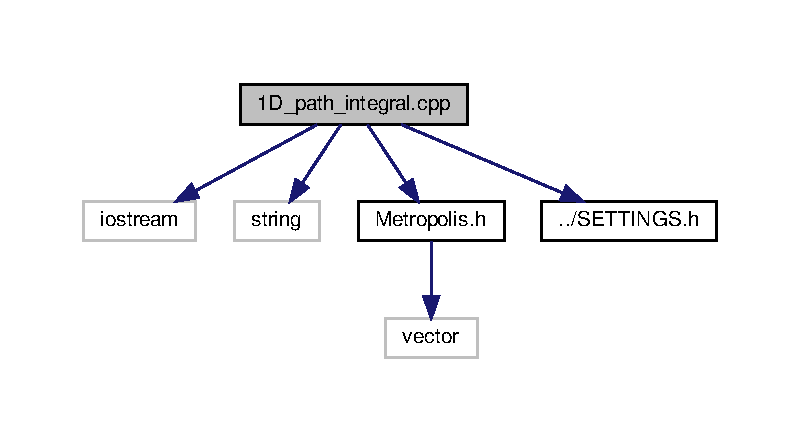
\includegraphics[width=350pt]{1D__path__integral_8cpp__incl}
\end{center}
\end{figure}


\subsection{Detailed Description}
Code to path integrate a 1D quantum system with Montecarlo method. 

In the main function, the physical parameters are set and the loop path integration is performed using the \hyperlink{classMetropolis}{Metropolis} algorithm, as implemented in the \hyperlink{classMetropolis}{Metropolis} class. Then, the requested observables are computed on the ensemble. Follow the comments in the source code of the \hyperlink{classMetropolis}{Metropolis} class for a more detailed description. 